% =========================================================================== %

\begin{frame}[t,plain]
\titlepage
\end{frame}

% =========================================================================== %

\begin{frame}{Fourier}
%
\begin{center}
	\includegraphics[width=.5\linewidth]{./gfx/xkcd-Fourier}
	
	That cat has some serious periodic components\\
	Source: \url{https://xkcd.com/26/}
\end{center}
%
\end{frame}

% =========================================================================== %

\begin{frame}
%
\begin{columns}[T]
\column{.33\linewidth}
\begin{Large}
	{Sound Waves}
	\vspace{6pt}
\end{Large}
%
\begin{itemize}
\item Recap: Fast pressure variations 
\item Hundreds to thousands of oscillations per second -- Hz or kHz
\item Pressure vs. time can be recorded by microphones
\item Time between two peaks: Period $T$
\item How many peaks per unit time: Frequency $\omega = \frac{2\pi}{T}$
\item Maximum pressure: Amplitude $A$
\end{itemize}
%
\column{.67\linewidth}
\begin{center}
	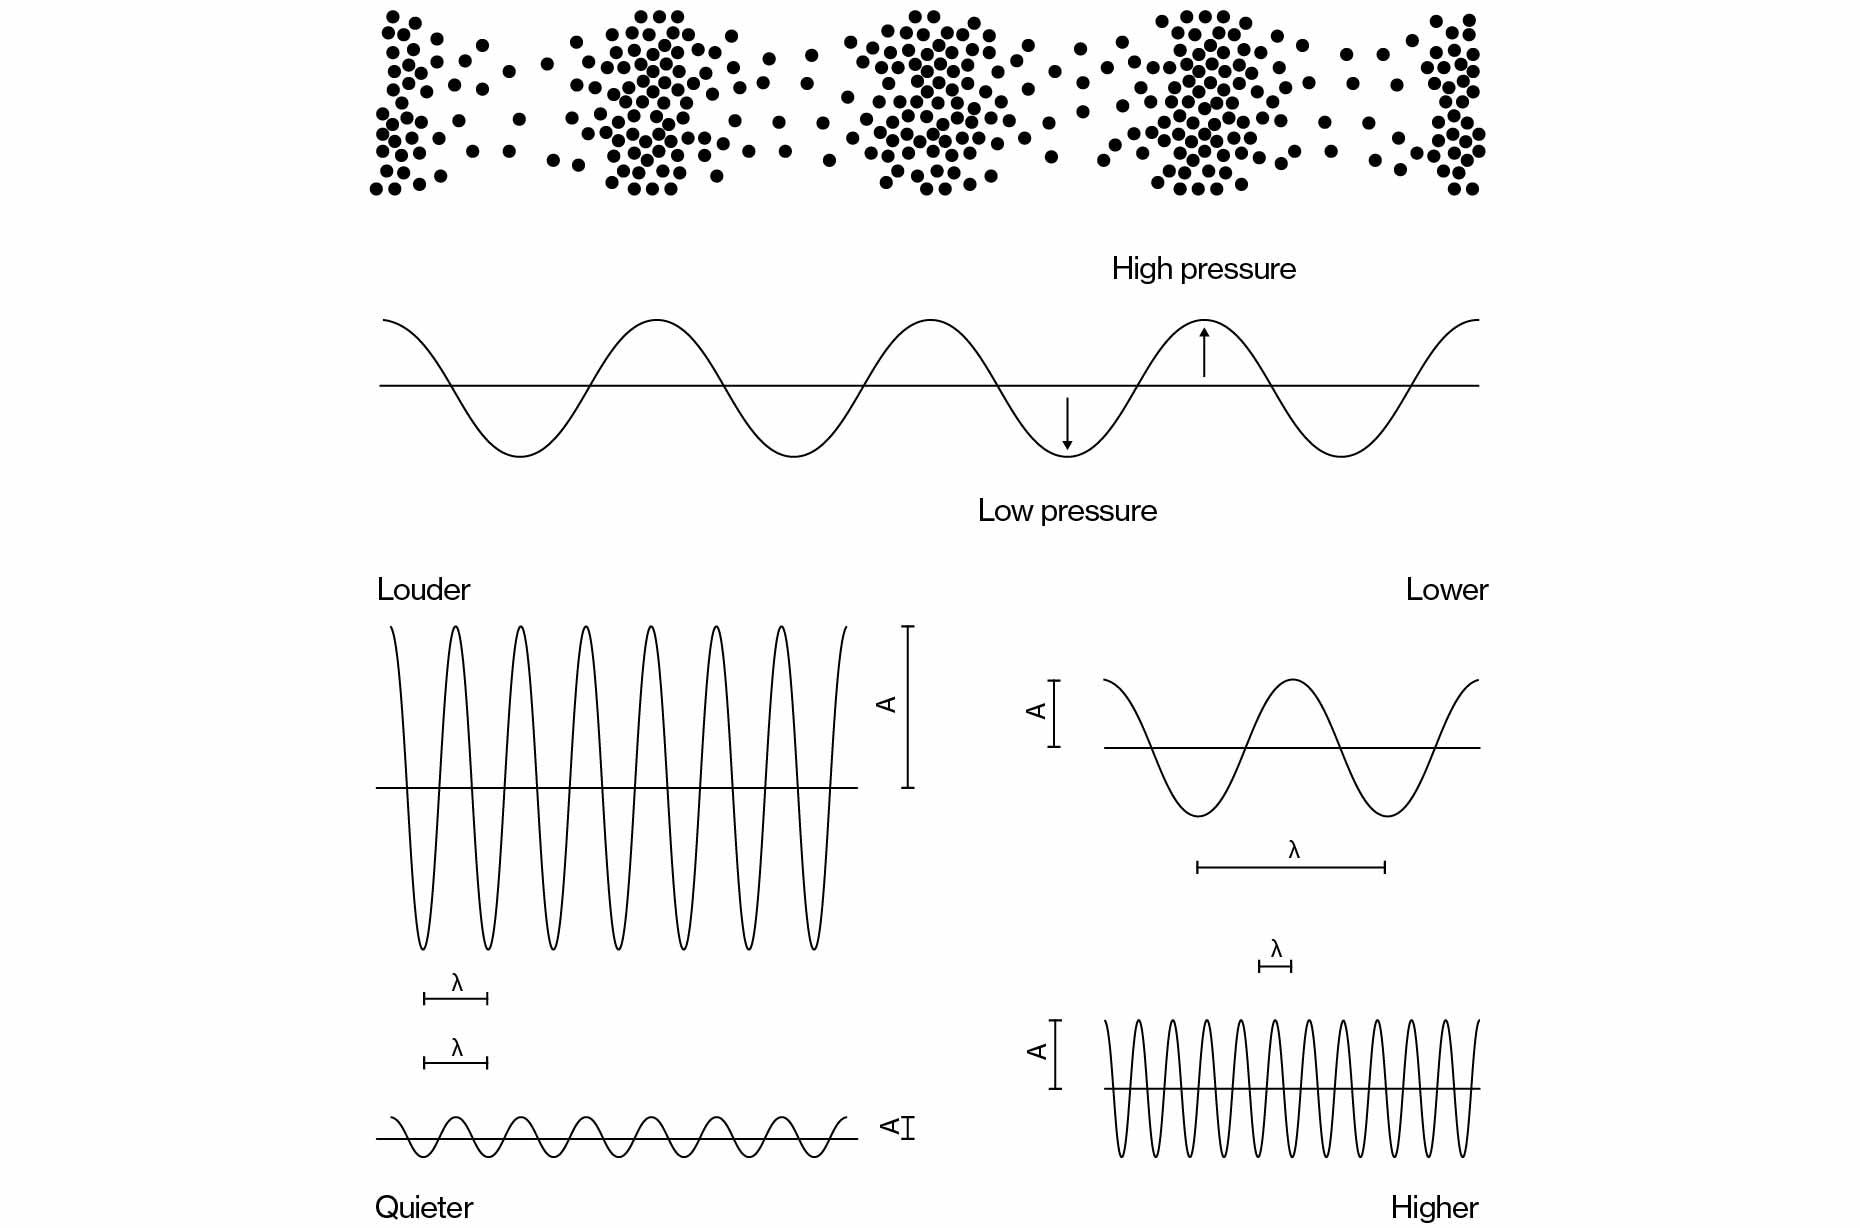
\includegraphics[width=\linewidth]{./gfx/soundwaves}
	\scriptsize
	\url{https://www.xal.com/de/know-how/schall-laerm/}
\end{center}
\end{columns}
%
\end{frame}

% =========================================================================== %

\begin{frame}[fragile]%{Superpositions -- Chords}
%
\begin{columns}[T]
\column{.67\linewidth}
\begin{codebox}[Example: Superposition]
\begin{minted}[fontsize=\scriptsize, linenos]{python3}
import matplotlib.pyplot as plt
import numpy as np

t = np.linspace(0, 2*np.pi, 300)
p1 = np.sin(X)
p2 = 1.0 * np.sin(1*t) +  0.3 * np.sin(5*t)

fig = plt.figure( figsize=(6, 12) )
drw1 = fig.add_subplot(211)
drw2 = fig.add_subplot(212)

drw1.plot(X, Y1)
drw2.plot(X, Y2)

fig.show()
\end{minted}
\end{codebox}
%
\column{.33\linewidth}
\begin{tcolorbox}[title=Output: Superposition]
	\begin{center}
	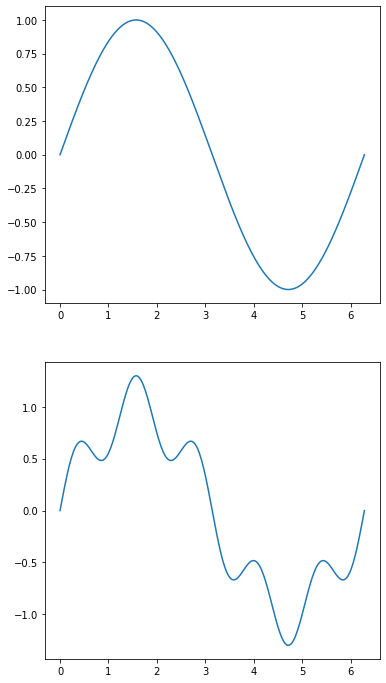
\includegraphics[width=.8\linewidth]{./gfx/sine-superposition}
	\end{center}
\end{tcolorbox}
\end{columns}
%
Two (or more) sounds can be played at the same time -- pressures sum up
%
\end{frame}

% =========================================================================== %

\begin{frame}{The Aim of Fourier Analysis}
%
\begin{center}
	\emph{Given the signal $p(t)$, can we reconstruct the amplitudes $A_1 = 1.0$ and $A_2 = 0.3$ together with the frequencies $\omega = 1$ and $\omega_2 = 5$?}
\end{center}
%
\begin{center}
	Yes, and this magic formula does the trick:
\end{center}
%
\begin{align*}
	A(\omega) = \frac{1}{2\pi} \int_{0}^{2\pi} p(t) \exp(-\iunit \omega t) \dd{t}
\end{align*}
%
This is the \emph{Fourier Transform} and it is what SciPy automatically computes with its \texttt{scipy.fft.fft} function.
%
\end{frame}

% =========================================================================== %

\begin{frame}{How does it work?}
%
We need to go through some concepts:
\begin{itemize}
\item Vectors and length of a vector
\item Scalar products
\item Functions as vectors
\item Euler's identity
\end{itemize}
%
\end{frame}

% =========================================================================== %

\begin{frame}
%
\begin{columns}[T]
\column{.7\linewidth}
\begin{Large}
	{Vectors and Lengths}
	\vspace{6pt}
\end{Large}
%
\begin{itemize}
\item Vector:
	\begin{itemize}
	\item \emph{ordered} list of mathematical objects (numbers)
	\item Python's \inPy{tuple}
	\end{itemize}
\item Length \emph{Euclidean} Norm
	\begin{itemize}
	\item What we usually understand as length
	\item Pythagorean theorem
	\item 2D: $\norm{\vec{a}} = \sqrt{x^2 + y^2}$
	\item 3D: $\norm{\vec{a}} = \sqrt{x^2 + y^2 + z^2}$
	\item $N$D: $\norm{\vec{a}} = \sqrt{\sum_i x_i^2}$
	\end{itemize}
\item Norm, general
	\begin{itemize}
	\item Something that behaves like a length
	\item (Almost) arbitrary function
	\item \enquote{Taxicab geometry}: $\norm{\vec{a}} = \sum_i \abs{x_i}$
	\end{itemize}
\end{itemize}
%
\column{.3\linewidth}
\begin{center}
	\tiny
	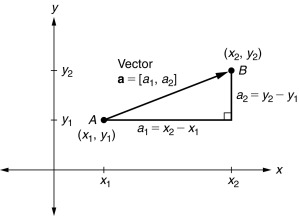
\includegraphics[width=\linewidth]{./gfx/pythagoras-2d}
	\url{https://www.sciencedirect.com/topics/mathematics/pythagorean-theorem}
	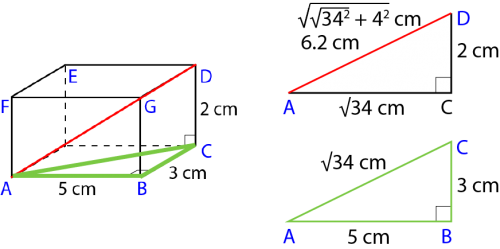
\includegraphics[width=\linewidth]{./gfx/pythagoras-3d}
	\url{https://mr-mathematics.com/pythagoras-theorem-in-3d-shapes/}
\end{center}
\end{columns}
%
\end{frame}

% =========================================================================== %

\begin{frame}[fragile]{Scalar Product}
%
\begin{columns}[T]
\column{.7\linewidth}
\begin{itemize}
\item A way of multiplying two vectors: $\vec{a} \cdot \vec{b} = \sum_i a_i \; b_i^*$
\item Sum of component-wise products
\item For technical reasons, take complex conjugate for RHS of scalar product
\item \enquote{Length of $\vec{a}$ in the direction of $\vec{b}$ in units of $\norm{b}$}
\item If $\vec{b}$ has length $1$ ($\norm{\vec{b}} = 1$):
	\begin{itemize}
	\item \enquote{$\vec{a} \cdot \vec{b}$ is the \emph{projection} of $\vec{a}$ in direction $\vec{b}$}
	\item Length of shadow when light source directly above (perpendicular to $\vec{b}$)
	\end{itemize}
\end{itemize}
%
\column{.3\linewidth}
\begin{center}
	\tiny
	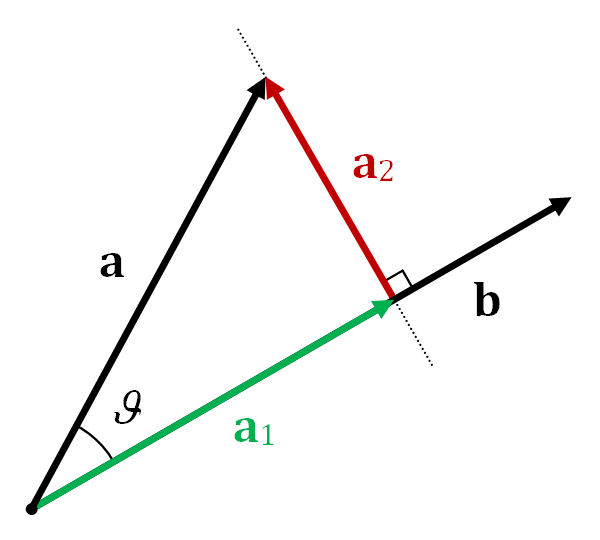
\includegraphics[width=\linewidth]{./gfx/Projection}
	\url{https://en.wikipedia.org/wiki/Vector_projection#/media/File:Projection_and_rejection.png}
\end{center}
\end{columns}
%
\end{frame}

% =========================================================================== %

\begin{frame}[fragile]
%
\begin{columns}[T]
\column{.7\linewidth}
\begin{Large}
	{Functions as Vectors}
	\vspace{6pt}
\end{Large}
%
\begin{itemize}
\item Function: infinitely many points
\item For each of infinitely many $x$, there is an $f(x)$
\item Imagine: (incomplete) list of only $N$ values
\item[\Thus] $N$-dimensional \emph{vector}!
\item Already allows a partial reconstruction of the original $f$
\item (Mathematically) possible: \emph{list all (infinitely many)} values
\item[\Thus] (Something like) a vector in infinite dimensions
\item \emph{Dear mathematicians, please don't fry me for this one}
\item Concepts defined on regular vectors still apply!
\item In particular: Scalar product aka projection!
\end{itemize}
%
\column{.3\linewidth}
\begin{center}
	\tiny
	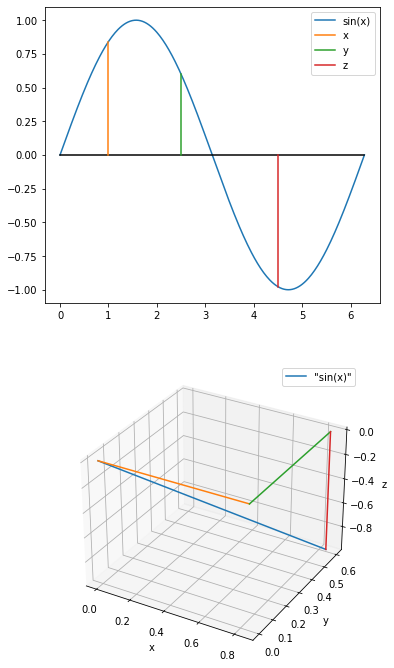
\includegraphics[width=\linewidth]{./gfx/sin-projection}
\end{center}
\end{columns}
%
\end{frame}

% =========================================================================== %

\begin{frame}{Fourier Analysis: Projection into the Frequency Domain}
%
\begin{columns}[T]
\column{.7\linewidth}
\begin{itemize}
\item Recall question: what is $A(\omega)$ when we have $p(t)$?
\item Amplitudes $A$ and frequencies $\omega$
\item One single oscillation: $f(t) = A \sin(\omega t)$
\item[\Thus] We need a scalar product!
	\[ A = \vec{p} \cdot \vec{f} \]
\item Can (almost) solve this with the means shown above!
\item Last (minor) problems:
	\begin{itemize}
	\item Require $\norm{f} = 1$
	\item How to sum up infinitely many values?
	\item How to deal with \emph{phase shifts}
	\end{itemize}
\end{itemize}
%
\column{.3\linewidth}
\begin{center}
	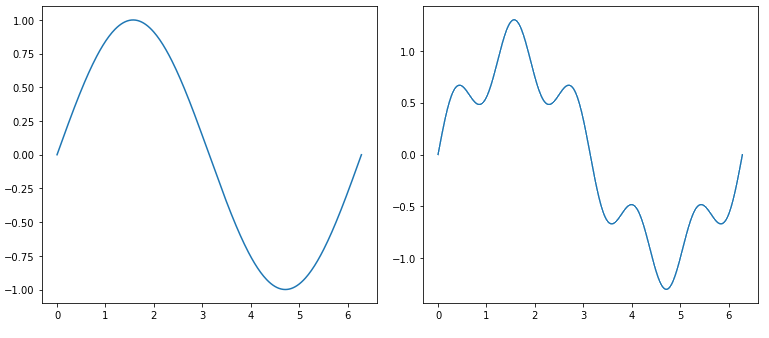
\includegraphics[width=\linewidth]{./gfx/sine-superposition-sbs}
	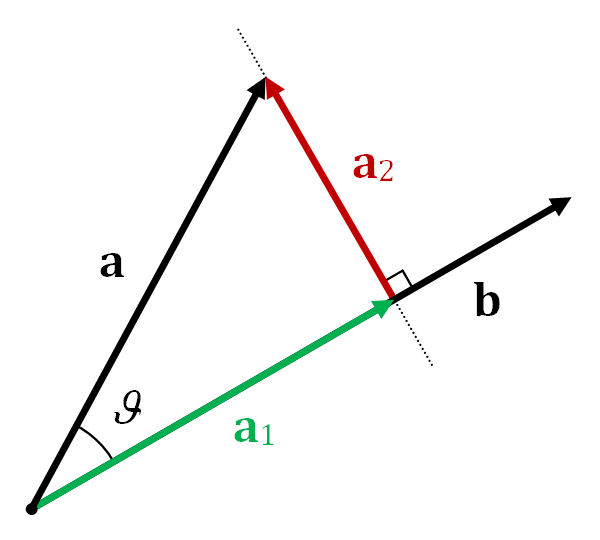
\includegraphics[width=.8\linewidth]{./gfx/Projection}
\end{center}
\end{columns}
%
\end{frame}

% =========================================================================== %

\begin{frame}[fragile]{Euler's Identity}
%
\[ \exp(\iunit \phi) = cos(\phi) + \iunit \sin(\phi) \]
%
\begin{minipage}{.49\linewidth}

\begin{center}
	\tiny
	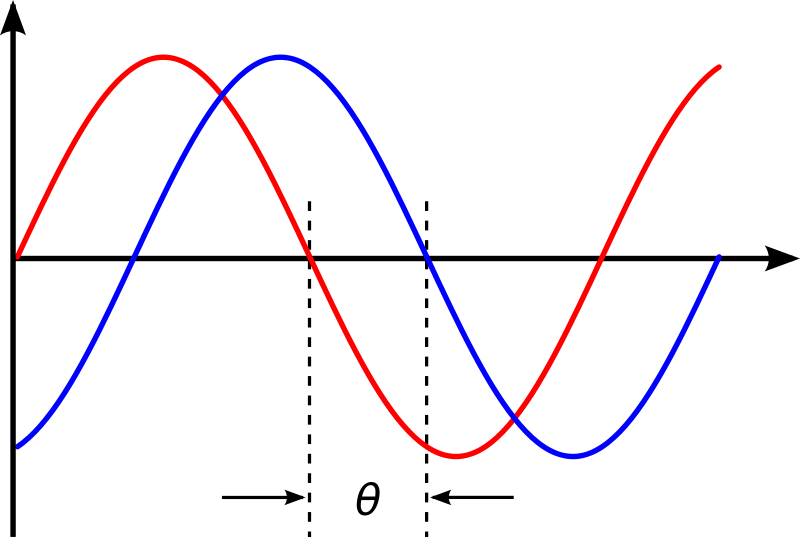
\includegraphics[width=.65\linewidth]{./gfx/phaseshift}
	\url{https://commons.wikimedia.org/wiki/File:Phase_shift.svg}
\end{center}
\end{minipage}
%
\begin{minipage}{.49\linewidth}

\begin{center}
	\tiny
	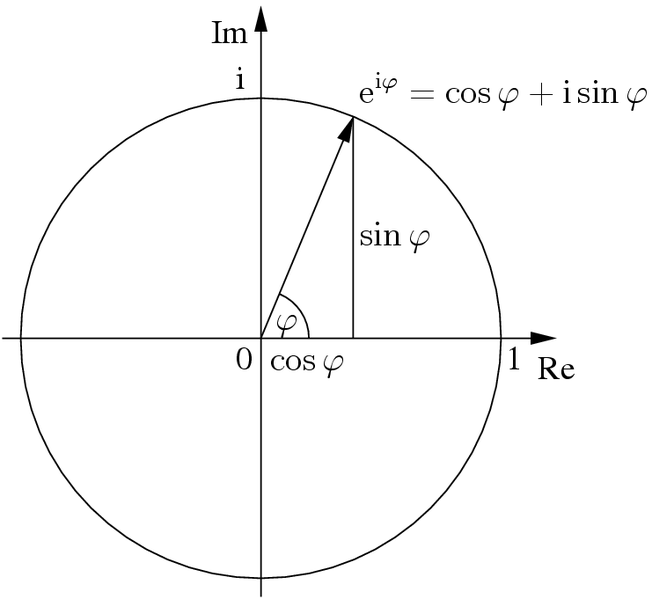
\includegraphics[width=.65\linewidth]{./gfx/EulerIdentity}
	\url{https://commons.wikimedia.org/wiki/File:Euler%27s_formula.svg}
\end{center}
\end{minipage}
%
Phase shifts can be represented by adding \emph{cosine} oscillations\\
Going from $\sin(\omega t)$ to $\exp(\iunit \omega t)$ allows to project onto both functions in one step
%
\end{frame}

% =========================================================================== %

\begin{frame}[fragile]{The last few problems}
%
\begin{itemize}
\item Length of the functions and normalization
	\begin{itemize}
	\item Remember: norm is (almost) arbitrary
	\item We can pick $\norm{f} = \int_0^{2\pi} \abs{f(x)} \dd{x}$ if we wish. (Which we do)
	\item For all $t \in \mathds{R} : \abs{ \exp(\iunit t) } = 1$
	\item[\Thus] $\norm{\exp(\iunit \omega t)} = 2\pi$
	\item[\Thus] Just divide result by $2\pi$
	\end{itemize}
\item Sum up infinitely many values
	\begin{itemize}
	\item Just go from summation to integration
	\item $\sum_i p_i \; f_i \rightsquigarrow \int p(x) f(x) \dd{x}$
	\end{itemize}
\item Put it all together, get our formula!
	\[ A(\omega) = \frac{1}{2\pi} \int_{0}^{2\pi} p(t) \exp(-\iunit \omega t) \dd{t} \]
\item Inverse is also possible
	\[ p(t) = \int_{0}^{\infty} A(\omega) \exp(\iunit \omega t) \dd{\omega} \]
\end{itemize}
%
\end{frame}

% =========================================================================== %

\begin{frame}
%
\begin{columns}[t]
\column{.7\linewidth}
\begin{Large}
	{Finite Difference Scheme}
	\vspace{12pt}
\end{Large}
%
\begin{itemize}
\item Assume, the world were \enquote{pixelated}
	\begin{itemize}
	\item Given a function $f(x)$, you cannot evaluate it for any $x$, but only for \emph{discrete} $x_i$
	\item \emph{Equidistant} points: $x_i = i \Delta x$
	\end{itemize}
\item Collection of all possible values: $f_i = f(x_i)$
\item[\Thus] Together they form a \emph{vector}
\item This is probably how you plotted most of your functions
\item One dimension for each pixel
\item[\Thus] Same idea as before
\item[\Thus] But: \emph{Finite} count of dimensions
\item[\Thus] And: Equidistant
\end{itemize}
%
\column{.25\linewidth}
\begin{center}
	\tiny
	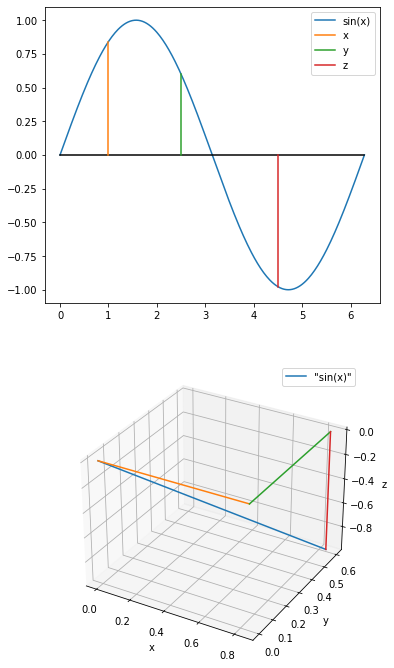
\includegraphics[width=\linewidth]{./gfx/sin-projection}
\end{center}
\end{columns}
%
\end{frame}

% =========================================================================== %

\begin{frame}{Finite Difference Scheme: Derivatives}
%
\begin{columns}[t]
\column{.6\linewidth}
\begin{itemize}
\item Standard definition of the derivative:\\
	$ \dv{x}f(x) = \lim_{h \to 0}\frac{f(x + h) - f(x)}{h} $
\item In pixelated world: $h \to 0$ not possible, but can only go down to $\Delta x$
\item Use \emph{Secant} instead as approximation\\
	$ \dv{x}f(x) \approx \frac{f(x + h) - f(x)}{h} $
\item Alternative: Backward definition of Derivative:\\
	$ \dv{x}f(x) \approx \lim_{h \to 0}\frac{f(x) - f(x - h)}{h} $
\item Alternative: \emph{Central Difference}:\\
	$ \dv{x}f(x) \approx \lim_{h \to 0}\frac{f(x + h) - f(x - h)}{2h} $
\end{itemize}
%
\column{.4\linewidth}
\begin{center}
	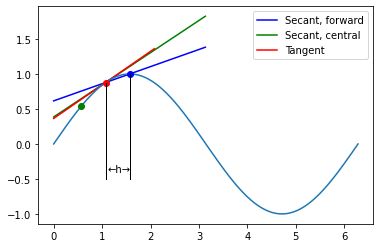
\includegraphics[width=\linewidth]{./gfx/SecantAndTangent}
\end{center}
%
\begin{itemize}
\item The central difference scheme mitigates the rounding error of the secant approximation a bit
\end{itemize}
\end{columns}
%
\end{frame}

% =========================================================================== %

\begin{frame}[fragile]{Finite Difference Scheme: Derivatives in Vectorized Functions}
%
\begin{itemize}
\item Formulae from before can be translated directly into code
\item Define \enquote{resolution} $h$
	\begin{itemize}
	\item Depends on physical unit of $x$-axis
	\item If none are present: make $h = 1$
	\end{itemize}
\item Compute all $f_i$:\\
	\inPy{vector = [f(i * h) for i in range(...)]}
\item Compute derivatives:\\
	\inPy{derivative = [(f[i+1] - f[i-1]) / (2*h) for i in range(1, len(i) - 1)]}
\item Note that \inPy{len(derivative) == len(vector) - 2}
\item Cf.: derivatives are only defined on \emph{open} intervals
\end{itemize}
%
\begin{hintbox}[Numerical Derivative is unstable]
\small
Compute the numerical derivative only where \emph{really} necessary -- it is very prone to numerical errors!
\end{hintbox}
%
\end{frame}

% =========================================================================== %

\begin{frame}{Differential Operator as Matrix Multiplication}
%
\begin{itemize}
\item Look at definition of finite/central difference:
	\[f'_i = \frac{f_{i+1} - f_{i-1}}{2h}\]
\item Can be expressed by a matrix:
	\begin{align*}
		D
	&=
		\frac{1}{2h}
		\mqty(
			   0   &    0    &    0   &    0   & \ldots &    &   0 \\
			  -1   &    0    &    1   &    0   & \ldots &    &   0 \\
			   0   &   -1    &    0   &    1   & \ldots &    &   0 \\
			\vdots &         & \ddots & \ddots & \ddots &    & \vdots \\
			   0   & \ldots  &  &           -1 &      0 &  1 &   0 \\
			   0   & \ldots  &  &              &     -1 &  0 &   1 \\
			   0   & \ldots  &  &              &        &    &   0
		)
	&
			\vec{f'}
		&=
			D\vec{f}
	\end{align*}
\end{itemize}
%
\end{frame}

% =========================================================================== %

\begin{frame}{Ordinary Differential Equations (ODEs)}
%
Imagine: Know how a system changes over time, but not its state itself at a given time.
\begin{itemize}
\item Notation
	\begin{itemize}
	\item Quantity $x(t)$
	\item Rate of change: $x(t)'$ or $\dot{x}(t)$ (\enquote{synonyms})
	\end{itemize}
\item Example: Radioactive decay
	\begin{itemize}
	\item Each $T$ units of time (seconds, years, ...), half of the atoms decay.
	\item[\Thus] How much of the substance is there after ${}^{t}/_T$ time units?
	\item state of the system: $N(t)$ atoms
	\item Rate of change: $N'\qty(\frac{t}{T}) = -\frac{1}{2} N\qty(\frac{t}{T})$
	\end{itemize}
\item Example: Constant Acceleration
	\begin{itemize}
	\item \emph{Velocity} $v$ is rate of change of position $x$
	\item \emph{Acceleration} $a$ is rate of change of velocity $v$
	\item \emph{Second} Derivative: rate of change of rate of change of position $\ddot{x} = a$
	\end{itemize}
\item[\Thus] How to find $N(t)$ and $x(t)$?
\end{itemize}
%
\end{frame}

% =========================================================================== %

\begin{frame}[fragile]
%
\begin{columns}[t]
\column{.6\linewidth}
\begin{Large}
	{Solving Differential Equations}
	\vspace{6pt}
\end{Large}
%
\begin{itemize}
\item \emph{Analytical} solutions
	\begin{itemize}
	\item Use your knowledge of analysis, algebra and black magic to somehow come up with a solution
	\item E.\;g.: $N(t) = N_0 \exp(-\lambda t)$ or $x(t) = x_0 + v_0 t + \frac{1}{2} at^2$
	\end{itemize}
\item \emph{Numerical} solutions
	\begin{itemize}
	\item Find the \emph{values} of the function (\enquote{in the pixelated world})
	\item Assume: $x(a + h) \approx x(a) + h \cdot x'(a)$
	\item Iteratively reconstruct $\vec{x}$ from jumping from $x_i$ to $x_{i+1}$ via $x'$
	\item Will be slightly off, but error depends on $h$
	\item Small $h$ \Thus small errors, but also many computations
	\end{itemize}
\item This is what \texttt{scipy.integrate.odeint} does!
\end{itemize}
%%
\column{.35\linewidth}
\begin{center}
	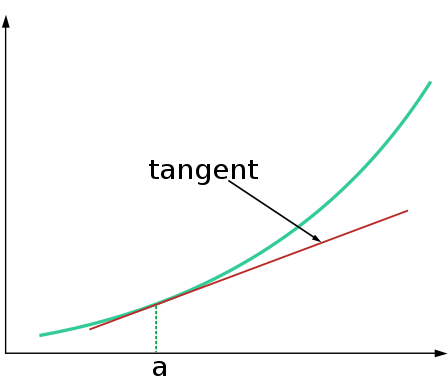
\includegraphics[width=\linewidth]{./gfx/tangent}
\end{center}
\begin{itemize}
\item (Plus tons of tricks to make this fast and accurate...)
\item[\Thus] Lecture \emph{Numerical Recipies} (Dr. Solbrig, each winter term)
\end{itemize}
\end{columns}
%
\end{frame}

% =========================================================================== %

\begin{frame}{Initial Conditions}
%
\begin{itemize}
\item For this method to work, the \emph{initial conditions} need to be known
\item \enquote{State of the system} at $t_0$
	\begin{itemize}
	\item Number of radioactie atoms, $N_0 = N(t_0)$
	\item Position and velocity, $x_0 = x(t_0), v_0 = v(t_0)$
	\end{itemize}
\item As many \emph{independent} information as the degree of the ODE
	\begin{itemize}
	\item In principle also possible: 2$^{\text{nd}}$ order ODE: $x_{\text{start}}$ and $x_{\text{final}}$
	\item Not compatible with the numerical approach
	\item Instead: All derivatives at $t_0$
	\end{itemize}
\end{itemize}
%
\end{frame}

% =========================================================================== %

\begin{frame}{Second Order ODEs}
%
\begin{itemize}
\item Often: Only expression for second (or higher) derivative given
\item Example free fall: $\dv[2]{x}{t} = \ddot{x} = g$
\item Includes two implicit first order ODEs:
	\begin{itemize}
	\item $ \dot{x}(t) = \dv{x}{t}(t) = v(t)$
	\item $\ddot{x}(t) = \dv{v}{t}(t) = g(t)$
	\end{itemize}
\item Recall: $v_0$ needs to be known
\item Get $v(t + \Delta t) = v(t) + h \dot{v}(t) = v(t) + h \ddot{x}(t) = v(t) + h \cdot g$
\item With $v(t + \Delta t)$, get $x(t + \Delta t)$ from same scheme
\item[\Thus] Simply find the implicit first order ODEs
\item[\Thus] Mere relabelling
\end{itemize}
%
\end{frame}

% =========================================================================== %

\begin{frame}{Vector-Valued ODEs}
%
\begin{itemize}
\item Function to be found can be more than [A number] at [a time]
\item Trajectory: coordinates via time
\item Formalism of ODEs still holds -- have vector valued ODE
\item $\vec{x'}(t) = \vec{f}(\vec{x})(t)$
\item Can be decomposed in components
	\begin{itemize}
	\item $x'_1(t) = f_1(\vec{x})(t)$
	\item $x'_2(t) = f_2(\vec{x})(t)$
	\item ...
	\end{itemize}
\item The $f_i$ can be treated independently from one another
\item Can be any order, even mixed order
\item Get a \emph{family} of systems of first order ODEs
\item Return $[x_1^{(1)}, x_1^{(2)}, ..., x_2^{(1)}, x_2^{(2), ...}]$
\end{itemize}
%
\end{frame}

% =========================================================================== %

\begin{frame}{Partial Differential Equations (PDEs)}
%
\begin{itemize}
\item Formal distinction: ODEs and PDEs
	\begin{itemize}
	\item ODEs comprise only derivatives wrt. \emph{one} variable (\eg wrt. time)
	\item PDEs comprise of derivatives wrt. \emph{several} variables
	\end{itemize}
\item Analytically: very difficult
\item Numerically: (sometimes) possible to solve them with the same approach
\item E.\;g.: Heat Equation
	\begin{itemize}
	\item $\pdv{T}{t} = \alpha \laplacian T$
	\item Nabla: $\nabla = \sum_i \hat{e_i} \pdv{x_i} $ -- Vector, comprising derivatives wrt. spatial coordinates
	\item Laplacian: $\laplacian = \sum_i \pdv[2]{x_i}$ -- Scalar, comprising second derivatives wrt. spatial coordinates
	\end{itemize}
\item No \enquote{mixing} between derivatives wrt. time and wrt. space
\item[\Thus] Work out $\laplacian T$, do numerical ODE approach for $\pdv{T}{t}$
\end{itemize}
%
\end{frame}